%DO NOT MESS AROUND WITH THE CODE ON THIS PAGE UNLESS YOU %REALLY KNOW WHAT YOU ARE DOING
\chapter{Design and Implementation} \label{Design andImplementation}
\section{Conceptual Design} \label{Conceptual Design}
\subsection{Fuzzy Inference System Design} \label{Fuzzy Inference System Design}
A fuzzy inference system (FIS) allows the use of fuzzy set theory to map inputs (etx, delay, hopcount, energy) to outputs (Quality). Due to it's simplicity in implementation we use the mamdani FIS.\\
\noindent A FIS can essentially be broken down into the following steps:\\
\vspace{-1cm}
\begin{itemize}
\item Fuzzification: take a crisp value input and determine its degree of membership (fuzziness) for the appropriate fuzzy sets.
\item Fuzzy inference: Apply combination rules to fuzzified inputs and compute a fuzzy output.
\item Aggregation: If an output depends on more than one rule, this step unifies all values into one.
\item Defuzzification: Convert the fuzzy output obtained at the previous step into a crisp value.
\end{itemize}
\subsubsection{Linguistic variables}
\noindent Node’s performances knowledge are represented as linguistic variables:\\
\vspace{-1cm}
\begin{itemize}
\item ETX - The expected number of required transmissions before a packet reaches the destination.
\item Delay - The average time for a packet to reach its destination.
\item Energy - The energy cost of the path, also energy of the node having the smallest remaining battery level on the path.
\end{itemize}
\subsubsection{Fuzzification process}
\begin{figure}[H]
\centering
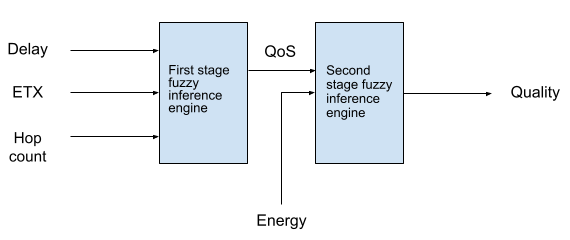
\includegraphics[width=100mm]{FIS.png}
\caption{fuzzy inference engine}
\label{fig:method}
\end{figure}
The fuzzification process is done in two stages to simplify the implementation.
\textbf{Stage 1:} The first stage combines etx, delay and hopcount into a compound metric Quality of Service (QoS). We use three membership functions for each linguistic variable, etx is divided into $ short $, $ average $, $ long $; delay is divided into $ small $, $ average $, $ high $; and finally hopcount is divided into $ near $, $ average $ and $ far $.\\
Figure 4.3 shows the membership functions for the 3 input parameters.
\begin{figure}[h!]
\centering
\subfigure[etx membership functions]
	{
	\label{fig:b}
	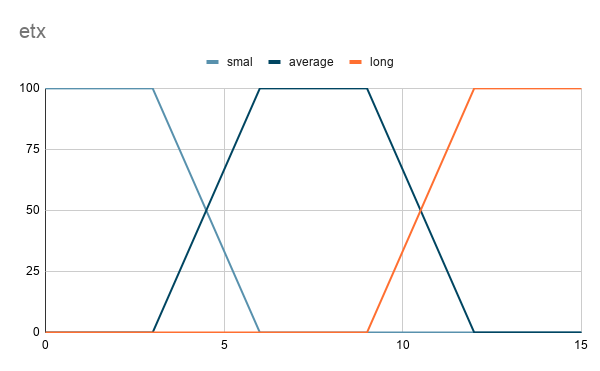
\includegraphics[width=50mm]{etx.png}
	}
\subfigure[hop count membership functions]
	{
	\label{fig:b}
	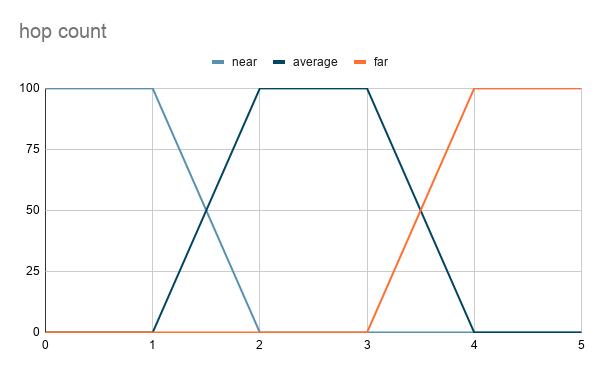
\includegraphics[width=50mm]{hop count.png}
	}
\subfigure[delay membership functions]
	{
	\label{fig:b}
	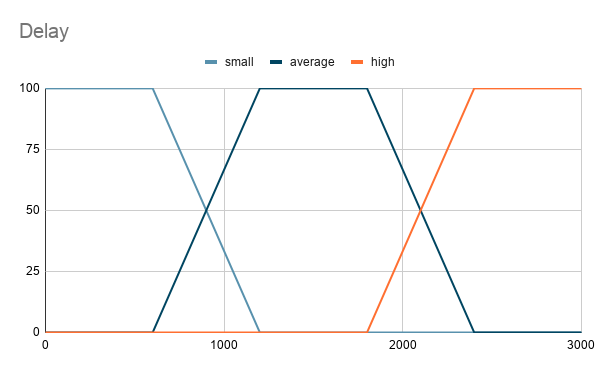
\includegraphics[width=50mm]{Delay.png}
	}
\caption{membership functions for first stage of fuzzification}
\label{fig:method}
\end{figure}
\noindent Table 4.1 shows the relationship between the three input linguistic variables for the computation of QoS.
\begin{table}[!ht]
\centering
\begin{tabular}{||c|c|c|c||}
\hline\hline
etx & delay & hop count & qos\\
\hline\hline
short & small & near & very fast\\
\hline
short & average & near & fast\\
\hline
short & high & near & average\\
\hline
short & small & average & fast\\
\hline
short & average & average & fast\\
\hline
short & high & average & average\\
\hline
short & small & far & fast\\
\hline
short & high & far & fast\\
\hline
short & high & far & average\\
\hline
average & small & near & fast\\
\hline
average & average & near & average\\
\hline
average & high & near & slow\\
\hline
average & small & far & fast\\
\hline
average & average & far & average\\
\hline
average & high & far & slow\\
\hline
long & small & near & average\\
\hline
long & average & near & slow\\
\hline
long & high & near & slow\\
\hline
long & small & average & average\\
\hline
long & average & average & slow\\
\hline
long & high & average & slow\\
\hline
long & small & far & average\\
\hline
long & average & far & slow\\
\hline
long & high & far & very slow\\
\hline\hline
  \end{tabular}
  \caption{QoS Output Metric}
\end{table}


\textbf{Stage 2:}We are combining the result obtained in the first stage (QOS) with the final metric to be  
considered i.e. ‘energy’. We are using trapezoidal membership function to represent energy . Energy is divided into low,medium and full subsections. The output of this stage is what we require that is ‘quality’. Quality of every parent is compared and the best parent is selected based on quality.\\
\noindent Table 4.2 shows how the output metric (quality) is decided based on the linguistic variables.\\
Figure 4.4 shows membership functions for Energy 
\begin{figure}[H]
\centering
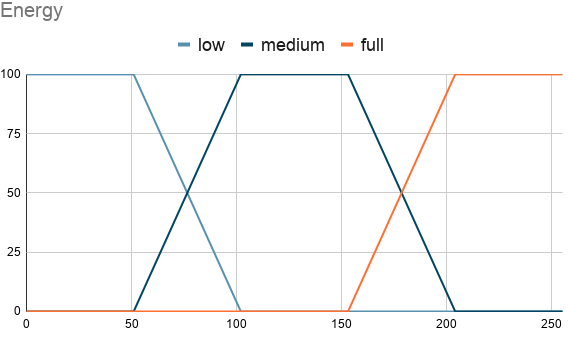
\includegraphics[width=70mm]{Energy.png}
\caption{membership function for Energy metric}
\end{figure}
\begin{table}[!ht]
\centering
\begin{tabular}{||c||c|c|c||}
\hline\hline
Qos / energy & low & medium & full\\
\hline\hline
very slow & awful & bad & average\\
\hline
slow & bad & degraded & average\\
\hline
average & degraded & average & acceptable\\
\hline
fast & average & acceptable & good\\
\hline
very fast & avrerage & good & excellent\\
\hline\hline
  \end{tabular}
  \caption{Quality Output Metric}
\end{table}

\section{Detailed Design} \label{Detailed Design}
\subsection{Implementation of Fuzzy Logic Controller in MATLAB} \label{Implementation of Fuzzy Logic Controller in MATLAB}
Fuzzy Logic Toolbox™ provides MATLAB® functions, apps, and a Simulink® block for analyzing, designing, and simulating systems based on fuzzy logic. The product guides you through the steps of designing fuzzy inference systems. Functions are provided for many common methods, including fuzzy clustering and adaptive neurofuzzy learning.\\
The toolbox lets you model complex system behaviors using simple logic rules, and then implement these rules in a fuzzy inference system. You can use it as a stand-alone fuzzy inference engine. Alternatively, you can use fuzzy inference blocks in Simulink and simulate the fuzzy systems within a comprehensive model of the entire dynamic system.
\subsubsection{Fuzzy Logic Designer} \label{Fuzzy Logic Designer}
Use the Fuzzy Logic Designer app or command-line functions to interactively design and test fuzzy inference systems. You can add or remove input and output variables. You can also specify input and output membership functions and fuzzy if-then rules. Once you have created fuzzy inference system, you can evaluate and visualize it.
\begin{figure}[h!]
\centering
\subfigure[Stage 1]
	{
	\label{fig:a}
	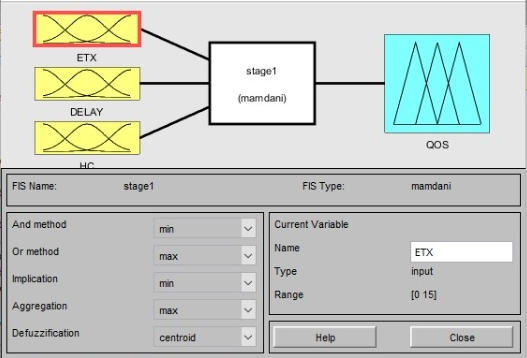
\includegraphics[width=100mm]{FuzzyControllerStage1.jpeg}
	}
\subfigure[Stage 2]
	{
	\label{fig:b}
	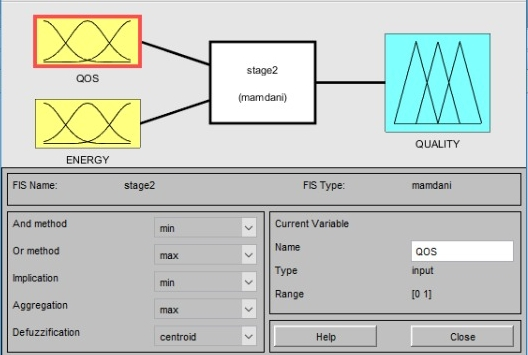
\includegraphics[width=100mm]{FuzzyControllerStage2.jpeg}
	}
\caption{Fuzzy Controller Designed in MATLAB}
\label{fig:method}
\end{figure}
\subsection{Requirements for implementing an OF in Contiki OS} \label{Requirements for implementing an OF in Contiki OS}
Some importtant files that have the gist of RPL are "rpl-config.h", "rpl-dag.c" and "rpl.c". Some important sections and parameters are mentioned here\\
\noindent\textbf{RPL\_DAG\_MC}
\begin{verbatim}
/* RPL_CONF_DAG_MC */
#ifdef RPL_CONF_DAG_MC
#define RPL_DAG_MC RPL_CONF_DAG_MC
#else
#define RPL_DAG_MC RPL_DAG_MC_NONE
#endif
\end{verbatim}
Here RPL metric container of the type using ETX and ENERGY are supported. However if you develop an objective function and an associated metric container can be supported.\\

\noindent\textbf{RPL\_OF}
\begin{verbatim}
/* RPL_CONF_OF */
#ifdef RPL_CONF_OF
#define RPL_OF RPL_CONF_OF
#else
#define RPL_OF rpl_mrhof
#endif
\end{verbatim}
The RPL\_CONF\_OF parameter configures the RPL objective function. ETX is the default objective function here. This should be defined to be the name of an rpl\_of object linked into the system image, e.g., rpl\_of0. Here you can also define it to be your own developed Objective function.\\

\noindent\textbf{RPL\_INIT\_LINK\_METRIC}
\begin{verbatim}
#ifndef RPL_CONF_INIT_LINK_METRIC
#define RPL_INIT_LINK_METRIC        5
#else
#define RPL_INIT_LINK_METRIC        RPL_CONF_INIT_LINK_METRIC
#endif
\end{verbatim}
This is the initial metric attributed to the link when ETX is unknown. It can be changed to any desirable value.\\

An objective function basically uses a link metric and has function which subject to a contraint tries to choose the best path for routing. To define a completely new Objective Function file(without modifying the existing one) the following functions must be defined in them. Also the makefile should be accordingly modified and care should be taken that your new file should not run into compilation and linking errors. \noindent Some of the API for RPL Objective function are:\\
\vspace{-1cm}
\begin{itemize}
\item $reset(dag)$: Resets the objective function state for a specific DAG. This function is called when doing a global repair on the DAG.
\item $neighbor\_link\_callback(parent, status, etx)$: Receives link-layer neighbor information.
\item $best\_parent(parent1, parent2)$: Compares two parents and returns the best one, according to the OF.
\item $best\_dag(dag1, dag2)$: Compares two DAGs and returns the best one, according to the OF.
\item $calculate\_rank(parent, base\_rank)$: Calculates a rank value using the parent rank and a base rank.
\item $update\_metric\_container(dag)$: Updates the metric container for outgoing DIOs in a certain DAG. If the objective function of the DAG does not use metric containers, the function should set the object type to $RPL\_DAG\_MC\_NONE.$
\end{itemize}

\subsection{Implementation of a FIS in C} \label{Implementation of a FIS in C}
\subsubsection{Fuzzification} \label{Fuzzification}
The required trapezoidal membership functions can be implemented in C using the following functions
\begin{verbatim}
unsigned int DOWN(unsigned int x1, unsigned int x2, unsigned int X) {
	return (TRUE * ((long)(X) - (long)(x2)))/((long)(x1) - (long)(x2));
}
unsigned int UP(unsigned int x1, unsigned int x2, unsigned int X) {
	return DOWN(x2, x1, X);
}
\end{verbatim}
The $DOWN()$ and $UP()$ functions implement the falling and rising edges of a trapezoidal membership function using the equation of a line with a maximum value of $TRUE=100$ and a minimum value of $0$\\
The membership functions over the entire range of input values are implemented using the $FIRST\_T\_NORM()$ for the lower values of the input range, $T\_NORM()$ for the central portion of the input and $LAST\_T\_NORM()$ is used for the higher values. Thus these produce the 3 trapezoidal membership functions required for all the input vairables in our project.
\begin{verbatim}
unsigned int FIRST_T_NORM(unsigned int b1, unsigned int b2, unsigned int px) {
	if (px <= b1) return TRUE;
	if (px > b1 && px <= b2) return DOWN(b1, b2, px);
	return FALSE;
}
unsigned int T_NORM(unsigned int b1, unsigned int b2, unsigned int b3, unsigned int b4, unsigned int px) {
	if (px <= b1) return FALSE;
	if (px > b1 && px <= b2) return UP(b1, b2, px);
	if (px > b2 && px <= b3) return TRUE;
	if (px > b3 && px <= b4) return DOWN(b3, b4, px);
	return FALSE;
}
unsigned int LAST_T_NORM(unsigned int b1, unsigned int b2, unsigned int px) {
	if (px <= b1) return FALSE;
	if (px > b1 && px <= b2) return UP(b1, b2, px);
	return TRUE;
}
\end{verbatim}
The membership functions as described in section \ref{Fuzzy Inference System Design} and illustrated in Figure 4.3, and Figure 4.4 for ETX, delay, hopcount and Energy can be implemented as:
\begin{verbatim}
#define ETX_MAX 15
#define ETX_B1 ETX_MAX / 5
#define ETX_B2 ETX_B1 * 2
#define ETX_B3 ETX_B1 * 3
#define ETX_B4 ETX_B1 * 4
#define etx_short(etx) FIRST_T_NORM(ETX_B1, ETX_B2, etx)
#define etx_avg(etx) T_NORM(ETX_B1, ETX_B2, ETX_B3, ETX_B4, etx)
#define etx_long(etx) LAST_T_NORM(ETX_B3, ETX_B4, etx)

#define DELAY_MAX 3000
#define DLY_B1 DELAY_MAX / 5
#define DLY_B2 DLY_B1 * 2
#define DLY_B3 DLY_B1 * 3
#define DLY_B4 DLY_B1 * 4
#define dly_small(dly) FIRST_T_NORM(DLY_B1, DLY_B2, dly)
#define dly_avg(dly) T_NORM(DLY_B1, DLY_B2, DLY_B3, DLY_B4, dly)
#define dly_high(dly) LAST_T_NORM(DLY_B3, DLY_B4, dly)

#define HOPCOUNT_MAX 5
#define HC_B1 HOPCOUNT_MAX / 5
#define HC_B2 HC_B1 * 2
#define HC_B3 HC_B1 * 3
#define HC_B4 HC_B1 * 4
#define hc_near(hc) FIRST_T_NORM(HC_B1, HC_B2, hc)
#define hc_avg(hc) T_NORM(HC_B1, HC_B2, HC_B3, HC_B4, hc)
#define hc_far(hc) LAST_T_NORM(HC_B3, HC_B4, hc)

#define ENERGY_MAX 255
#define ENG_B1 ENERGY_MAX / 5
#define ENG_B2 ENG_B1 * 2
#define ENG_B3 ENG_B1 * 3
#define ENG_B4 ENG_B1 * 4
#define energy_low(eng) FIRST_T_NORM(ENG_B1, ENG_B2, (eng))
#define energy_medium(eng) T_NORM(ENG_B1, ENG_B2, ENG_B3, ENG_B4, (eng))
#define energy_full(eng) LAST_T_NORM(ENG_B3, ENG_B4, (eng))
\end{verbatim}
\subsubsection{Fuzzy Inference} \label{Fuzzy Inference}
The $min()$ and $max()$ functions which are used to evaluate the antecident in the fuzzy rule base are implemented using simple macros such as
\begin{verbatim}
#define max(a, b) x>y?x:y
#define min(a, b) x<y?x:y
\end{verbatim}
The fuzzy rulebase can then be represented using max and min equivalents for AND and OR logic in the if-them statements
\subsubsection{Aggregation} \label{Aggregation}
Aggregation is done using the Center of gravity method for QoS and Quality respectively